\taskpic{
    Массивный клин с углом $\theta$ в основании стоит на гладкой поверхности. На клин налетает упругий шарик, скорость
    которого параллельна поверхности стола. Шарик отскакивет от клина и через некоторое время приземляется на него в точке
    первого контакта. Найдите отношения масс шарика и клина.
}{
    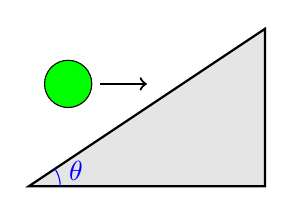
\begin{tikzpicture}
        \draw[thick, fill = gray!20] (0, 0) -- (3, 2) -- (3, 0) -- cycle;
        \draw (0.6, 0.2) node[blue] {$\theta$};
        \draw[blue] (0.4, 0) arc (0:35:0.4);
        \draw[fill = green] (0.5, 1.3) circle (0.3cm);
        \draw[thick, ->] (0.9, 1.3) -- ++(0.6, 0);
  \end{tikzpicture}
}
% Physics Challenges, TPT, November 2006
% в системе центра масс всё выглядит сравнительно просто